\chapter{Methodology}\label{method}
\label{Methodology}
In previous chapters we introduced our research problem, listed and explained the solution options with the theoretical background. In this chapter we shall try to explain our practical approach for carrying out the research along with the software development required to support the experimentation and data analysis for our research. On a practical level following were some major tasks that were required to fulfil scope of our research.
\begin{itemize}
\item Understanding energy efficiency, smart grids and available data.
\item Requirement engineering and use case preparation.
\item Understanding Data Analytics ecosystem, evaluating the big data tools and solutions.
\item Exploratory data analysis and selection of algorithms and data analysis tools with respect to use cases. 
\item Developing an end to end big data analytics platform.
\item Data collection, storage and preprocessing.
\item Use case specific data analysis and evaluation of results.
\item Visualization of results 
\item Documentation of the research, process, software development and results.
\end{itemize}
Some of these tasks were required to be performed in a sequential way e.g. requirement engineering and evaluation of big data tools were required before developing the big data analytics platform or selecting the algorithms. Similarly we need to have results before visualizations could be created. On the other hand some of the tasks could have been executed in parallel. For example the documentation was an ongoing process along with all other tasks. Similarly literature review for understanding each component of our research was also an ongoing process through the time line for this thesis. The regardless of sequential and parallel tasks we need to iterate for continuous improvement.

To tackle these challenges we needed a methodology that can support sequential and parallel task execution with support for iterations to improve. Like most of scientific researches, fail fast and small to succeed was the key for us. In the list of tasks mentioned above. Most of them requires conceptualization and tested quickly using rapid prototyping. Taking it as a software development task initially, we had some candidate models such as water fall model,agile development model, spiral model and incremental model etc. Here we shall briefly discuss the advantages and disadvantages in context to our research project. 
\begin{itemize}
\item \textbf{Waterfall model} offered the simplest approach of requirement engineering, design, implement, test and operate our research. How ever it is inherently sequential and had weak support for iterations.
\item \textbf{Agile development model} Agile methodology\cite{martin2003agile} is rapid, iterative and supports quick prototyping but it requires additional communication and management overhead like scrum meetings. Managing it along with stakeholders like VTT and CIVIS projects was very hard.
\item \textbf{Spiral Model} is a risk driven process model.It supports prototyping, provides good way of avoiding major failure risks, it is iterative. However it needs a lot of resources during planning phase specially when the spiral keeps growing in size. It is usually very successful for large projects but it has over heads for small projects like our thesis research. We shall be discussing more about using parts of the spiral model later in this chapter.
\item \textbf{Incremental model} relies on small incremental steps with each step consist of independent design, implement and test phase. In the begining, Incremental model was the best fit among other candidate models for our thesis research.We were able to prototype small functional units of the big data analytics platform very quickly while independently working on the use cases. However during platform development and data analysis part. It has started creating integration over heads. For example integrating two different data processing tools together for a single use case becomes difficult  when they were configured in two different incremental steps.  
\end{itemize}
Learning from the problems that we face from  incremental model we altered our approach to adapted version of another very flexible software research and development methodology known as ``Kumiega-Van Vliet Trading System Development Methodology''\cite{kumiega2008software}.

\section{Kumiega-Van Vliet Model}\label{kvvm}   
      
Kumiega-Van Vliet Trading System Development Methodology \((K|V)\) was developed in 2008 for software development required specifically for trading systems. It is the combination of three general purpose software and new product development models i.e. waterfall model, spiral model and stage gate model. We have already explained the waterfall and spiral models. Stage gate model consists of stages e.g. scoping, development, implementation, testing etc. Each stage or combination of stages can be controlled with an approval gate. Process can not move from a stage to other stage if the gate in between them is not approved.This model provides a good control over the development model to ensure quality. However it may cause delays because of the organizational hierarchies dictating the gates.

 \((K|V)\) model tries to overcome the short comings of these three models by combining them to a single paradigm for trading system development\cite{kumiega2008software}. In spiral model in start smaller time is allocated to four basic steps i.e. research planning implementation and test. These four steps can be performed again and again in cycles. To avoid spiral to grow two much after each cycle a stage gate controls if process can be passed to next stage or it needs to be sent back to perform another cycle in same stage. Just like waterfall there can be number of stages. But for continuous improvements process there is an iteration channel available unlike traditional waterfall model.
 \section{Adaptation of Kumiega- Van Vliet Model}\label{adaptation}
 \((K|V)\) model is designed for software research  and development in domain of financial services. With the built in stage gate controls it requires some scale of hierarchical organizational structure to support the model. For our highly academic research case we have made certain adjustments. The most notable adaptation was to use deliverables and team reviews of respective deliverables as the main control for moving from one stage to other instead of stage gate approvals in \((K|V)\) model. The waterfall model alike stages helped in keeping our focus on the solution for our problem statement. The spiral model cycles enabled us to iterate within a stage and improve the deliverables quality. Typically the decision of additional cycles was based on the feedback during the team review sessions. The inter stage iteration channels helped us in improving our overall quality. The lessons learnt or the new directions identified during one iteration was include in the scope of research for next iteration. It also allowed us to include supplementary topics in our scope without losing focus on mandatory issues.
 
 In our approach, we have divided complete scope of research in four basic stages. Within each stage we had four steps. These intera stage steps were different for each stage. These steps were corresponding to the main tasks that we discussed in start of this chapter. A typical intra stage cycle ended with a set of deliverables. The deliverables were reviewed in a team review session. If required the other stockholders like VTT was also involved in some of the review meetings. We shall be discussing it in details when we describe our stage wise proceedings. At end of each review session a decision was made to either move to next stage or try to imrove via additional cycle. Using all four intra stage steps for additional cycles was not a must. This was another minor adaptation to the \((K|V)\) model. Similarly iterations were were mostly initiated after stage three. There were three major iterations. During the iterations change of deliverables were not mandatory. However in practice it was observed that iteration had caused some major or minor changes in stage deliverables as well. Small informal team structure reduced management and communication efforts. This also helped in rapid processing during iterations. Figure~\ref{fig:kv} illustrates our approach with the adapted version of \((K|V)\) model. Stage by stage description of our research methodology is explained in next section.   
 \begin{figure}[!h]
   \begin{center}
     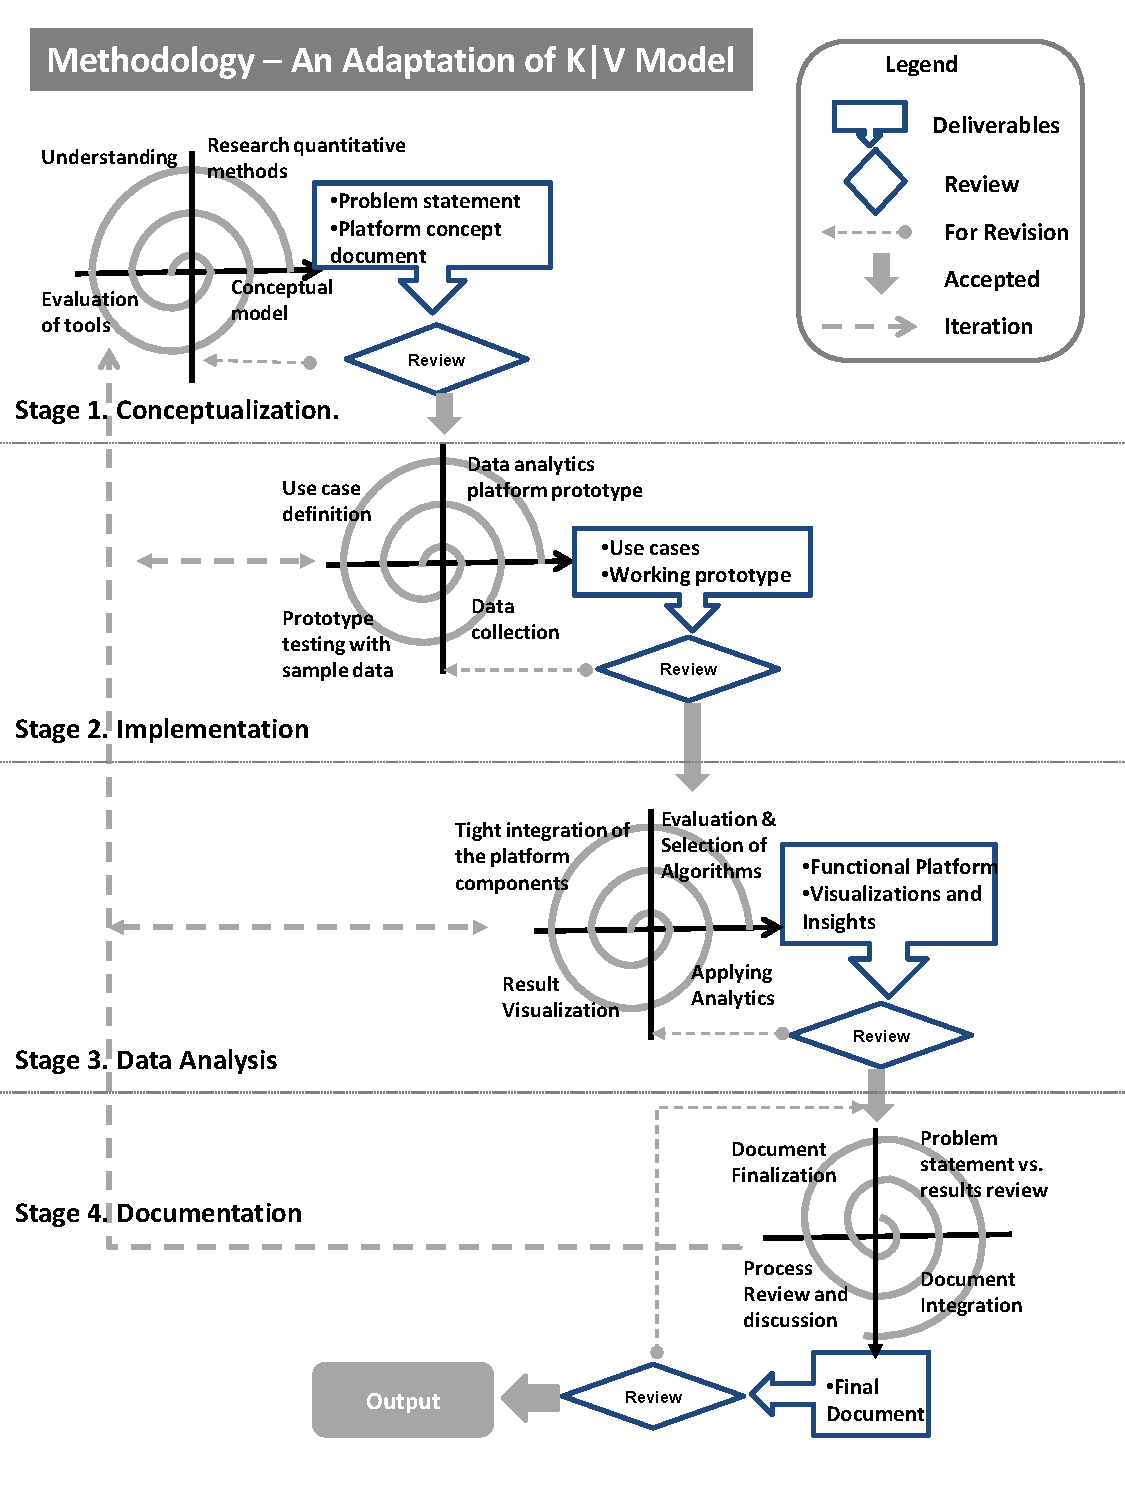
\includegraphics[width=\textwidth]{images/kv_method.pdf}
     \caption{Methodology, An Adaptation of \(K|V\) Model}
     \label{fig:kv}
   \end{center}
 \end{figure} 
\section{Stages, steps and cycles}\label{stages} 
We have already mentioned that there were four stages with each having four respective steps. Each stage was controlled via deliverables review sessions in a stage gate manner. While inside a stage, steps were executed in spiral cycles. First cycle of the spiral had to pass through the four steps. The additional cycles are initiated if the further improvements are decided for deliverables in review session. All Four steps were not mandatory for additional cycles. In this section we shall be listing and describing the stages along with respective steps. We shall be highlighting some major cycles and deliverables. However the iterations will be discussed in next section. Figure ~\ref{fig:kv} will be our main reference through out this section. In this section we shall mention some functional components of our project e.g. logical architecture, data processing tools and algorithms etc. Details for these functional components will be given in later part of this document.
\subsection{Stage 1. Conceptualization } \label{concept}
In start our research problem was mainly concerned about processing large volumes of data coming from smart metering devices and understand the consumption patterns. So the primary focus of the conceptualization stage was to describe our problem in detail, understand important factors related to it, find and evaluate methods and tools to solve the problem. The stage had following four steps.
\subsubsection{Step 1. Understanding} 
From the start, our research had two focus areas i.e. energy consumption and big data . The main purpose of this step was to understand important concepts related to these topics. Follwoing are some main activities performed during this step.
\begin{itemize}
\item Intensive literature review.
\item Participation in CIVIS project Helsinki- Use case workshop 26-27 January 2014. It gave good insights about ecological and social factors effecting energy production, distribution and consumption.
\item Participation in VTT Green Campus Initiative Introduction session.
\item Discussions and informal interviews with VTT's project lead for Green Campus Initiative.
\item Aalto University courses.
	\begin{enumerate}
	    \item Scalable Cloud Computing, as a good introduction to parallel batch processing and its uses for big data processing.
	    \item Information Visualization, as an introduction to effective communication through data visualization.
	  \end{enumerate}      
\end{itemize}

Literature review had been a constant step through out this stage, cycles, and iterations.
\subsubsection{Step 2. Research quantitative methods} 
This step involved finding and evaluating the various quantitative methods used for measuring energy consumption and benchmarking energy efficiency. Data aggregation methods like daily, monthly consumption, and average consumption etc were evaluated. Identification and theoretical evaluation of advance analytical methods was also performed during this step.
\subsubsection{Step 3. Conceptual Model}\label{cmodel}
This step was dedicated for finding available open source solutions to make a conceptual model for an end to end big data analytics. This step was mandatory for the big data platform concept paper deliverable. This step was also repeated during various iterations, whenever change was required in data platform.
\subsubsection{Step 4. Evaluation of Tools}
This step was in pair with \ref{cmodel}. All the tools listed in conceptual model were tested during this step. A checklist of evaluated and selected tools was maintained. This list is available as annex???

\subsubsection{Delivearbles of stage 1}
There were two deliverables of this stage
\begin{enumerate}
\item Problem Statement. first two steps of this stage were the main contributors for this deliverable.
\item Platform concept document. A document as result of step 3 and 4 of this stage. 
\end{enumerate}

\subsubsection{Stage 1 cycles}
In this stage we observed two cycles i.e. cycle for producing the required deliverables and one additional cycle for modification of platform concept document. The main modification in additional cycle was the replacement of application frame work with an architecture diagram to clarify.
\subsection{Stage 2. Implementation}
This stage mainly includes requirement engineering and intensive software development to prototype and test the big data platform described in concept paper as a deliverable from stage 1. This stage had following four steps.
\subsubsection{Use case definition} 
In this step, Based on the knowledge gained from stage 1. we decomposed our problem statement into lower level requirements that can be practically implemented using big data platform concept. Use cases went through several iterations. Details of iterations will be discussed later in this chapter. However here we shall list the final list of use cases.
\begin{enumerate}
\item Understanding the seasonal energy usage patterns and its sensitivity with outside temperature.
\item Understanding characteristics of building using daily energy consumption pattern.
\item Calculate the base load of the building to identify non user consumption of buildings
\item Classify building on basis of energy efficiency and analyse seasonal shifts in this classification.
\item Predict daily energy consumption of various house hold devices on basis of previous consumption pattern. 
\end{enumerate}
 

  

 
